%% Based on:

%%%%%%%%%%%%%%%%%%%%%%%%%%%%%%%%%%%%%%%%%
% a0poster Portrait Poster
% LaTeX Template
% Version 1.0 (22/06/13)
%
% The a0poster class was created by:
% Gerlinde Kettl and Matthias Weiser (tex@kettl.de)
%
% This template has been downloaded from:
% https://www.latextemplates.com/template/a0poster-portrait-poster
%
% License:
% CC BY-NC-SA 3.0 (http://creativecommons.org/licenses/by-nc-sa/3.0/)
%
%%%%%%%%%%%%%%%%%%%%%%%%%%%%%%%%%%%%%%%%%


%----------------------------------------------------------------------------------------
%	PACKAGES AND OTHER DOCUMENT CONFIGURATIONS
%----------------------------------------------------------------------------------------

\documentclass[a0,portrait]{a0poster}

\usepackage[backend=biber]{biblatex}
\addbibresource{bib/main.bib}
\addbibresource{bib/comp.bib}
\addbibresource{bib/misc.bib}
\AtEveryBibitem{
  \clearfield{issn}
  \clearfield{month}
  \clearfield{doi}
  \clearfield{note}
}


\usepackage{multicol} % This is so we can have multiple columns of text side-by-side
\columnsep=100pt % This is the amount of white space between the columns in the poster
\columnseprule=3pt % This is the thickness of the black line between the columns in the poster

\usepackage[svgnames]{xcolor} % Specify colors by their 'svgnames', for a full list of all colors available see here: http://www.latextemplates.com/svgnames-colors

% \usepackage{newtxtext} % Use the times font for text, newer flavor
% \usepackage{helvet}
% \usepackage{mathpazo}
\renewcommand{\familydefault}{\sfdefault} % sans serif font

\usepackage{graphicx} % Required for including images
\graphicspath{{img/}} % Location of the graphics files
\usepackage{booktabs} % Top and bottom rules for table
\usepackage[font=small,labelfont=bf]{caption} % Required for specifying captions to tables and figures
\usepackage{wrapfig} % Allows wrapping text around tables and figures
\usepackage{amsfonts, amsmath, amsthm, amssymb} % For math fonts, symbols and environments

\usepackage{physics}
%\usepackage[T1]{fontenc}
\usepackage{setspace}

\setlength{\fboxsep}{2.5mm}

\usepackage{bbm}

\usepackage[top=2.8cm,right=2.8cm,bottom=2.8cm,left=2.8cm]{geometry}

\usepackage{lipsum}

% %% https://tex.stackexchange.com/a/366170
% \makeatletter
% \renewenvironment{abstract}{%
%   \begin{center}%
%     {\bfseries \large\abstractname\vspace{\z@}}
%   \end{center}%
%   \quotation
% }
% \makeatother

%----------------------------------------------------------------------------------------
% FROM tex/lib.tex
%----------------------------------------------------------------------------------------
% TODO: DRY
\newcommand{\term}[1]{\emph{#1}}
\newcommand{\idop}{\mathbbm{1}}           % Identity operator
\newcommand{\hilb}[1]{\mathcal{#1}}       % Hilbert space
\newcommand{\setof}[1]{\left\{#1\right\}}
\newcommand{\ox}{\otimes}
%
%% Allows better formatting than \underset
%% https://tex.stackexchange.com/a/130553
\DeclareMathOperator*{\repr}{\equiv}      % represented in a basis, or "has components..."
%
\renewcommand{\op}{\hat}                  % overwriting physics \op = \ketbra
\newcommand{\eqbydef}{\coloneqq}
%\newcommand{\eqbydef}{\triangleq}
\newcommand{\superop}{\mathcal}
%
\newcommand{\smallback}{\hspace{-0.115em}}
\newcommand{\largeback}{\hspace{-0.365em}}
%
\newcommand{\dket}[1]{\left.\left| #1 \right\rangle\smallback\right\rangle}
\newcommand{\Dket}[1]{\left.\left| #1 \right\rangle\largeback\right\rangle}
% and similar...
\newcommand{\dbra}[1]{\left\langle\smallback\left\langle #1 \right|\right.}
\newcommand{\dbraket}[2]{\left\langle\smallback\left\langle #1 \middle| #2 \right\rangle\right.}
\newcommand{\bradket}[2]{\left.\left\langle #1 \middle| #2 \right\rangle\smallback\right\rangle}
\newcommand{\dbradket}[2]{\left\langle\smallback\left\langle #1 \middle| #2 \right\rangle\smallback\right\rangle}
\newcommand{\dketdbra}[2]{\left| #1 \left\rangle\smallback\left\rangle \smallback \right\langle\smallback\right\langle #2 \right|}

%\definecolor{boxedcolor}{RGB}{32, 48, 32}
\definecolor{maincolor}{RGB}{16, 48, 16}
%\definecolor{boxedcolor}{maincolor}


%\renewcommand{\abstractname}{\large Abstract} % abstract hacks

\begin{document}

%----------------------------------------------------------------------------------------
%	POSTER HEADER
%----------------------------------------------------------------------------------------

% The header is divided into two boxes:
% The first is 75% wide and houses the title, subtitle, names, university/organization and contact information
% The second is 25% wide and houses a logo for your university/organization or a photo of you
% The widths of these boxes can be easily edited to accommodate your content as you see fit
\begin{minipage}[c]{0.70\linewidth}
\VeryHuge\color{NavyBlue}\textbf{It's $\ket{1}$ o'clock} \color{Black}\\[0.5cm] % Title
\huge\textit{Relational Time and Applications}\\[1cm] % Subtitle
\huge University College Cork, School of Physics\\[0.66cm] % University/organization
\Large{Guido De Rosa, Andreas Ruschhaupt}

\end{minipage}%
%
\begin{minipage}[t]{0.30\linewidth}

\includegraphics[width=18cm]{ucc_logo.pdf}\\  %% vector, from original SVG
\end{minipage}

\vspace{2cm} % A bit of extra whitespace between the header and poster content

%----------------------------------------------------------------------------------------

\begin{multicols}{2} % This is how many columns your poster will be broken into, a portrait poster is generally split into 2 columns

%----------------------------------------------------------------------------------------
%	ABSTRACT
%----------------------------------------------------------------------------------------

\color{Navy} % Navy color for the abstract

\section*{Abstract}
{Time} in quantum mechanics is generally regarded as a (classical) parameter \cite{TQM1, TQM2}.
%
The \emph{Page and Wootters} (PaW) model
describes time as a quantum observable with its associated self-adjoint operator.
%
Within the formalism, \emph{evolution} {emerges} in terms of \emph{entanglement} between non-interacting subsystems
of a “universe” in a stationary state.
%
An opportune subsystem can be identified as a “clock” for the “rest”
of it \cite{Lloyd:Time}.
%
In this work~\cite{DeRosaMSc}, \emph{discrete} clocks are implemented,
and PaW predictions are compared to
standard quantum mechanics for some simple systems.
%
Non-unitary evolution is also studied, in relation to \emph{absorptive} detector models \cite{RuschhauptAbsorption}.
A time-of-arrival statistical distribution is derived.

\setlength{\parindent}{2em} % Default is 15pt.

%----------------------------------------------------------------------------------------
%	INTRODUCTION
%----------------------------------------------------------------------------------------

\color{SaddleBrown} % SaddleBrown color for the introduction

%\large

\section*{Historical background: The Pauli Objection}

``[As] a matter of fact, a number of time observables are already routinely measured in
laboratories, for example arrival times in time-of-flight experiments, but the theoretical foundation
of these measurements is still being discussed'' \cite{TQM1}.
%
``The Schr\"odinger's equation says that the Hamiltonian is the generator of time translations. This seems
to imply that any reasonable definition of time operator must be conjugate to the Hamiltonian''~\cite{Maccone:Pauli}.

Despite these considerations,
the idea of
such time operator
is hindered by the \emph{Pauli's argument} \cite{PauliFootnote}.
The objection
is that
an operator~$\hat{T}$,
canonically conjugate to the Hamiltonian $\hat{H}$,
i.e.
$
  \label{THcommutator}
  [\hat{T}, \hat{H}] = i\hbar
  \text{,}
$
implies that the spectrum of \emph{any} Hamiltonian must be the whole real line $\mathbb{R}$
(thus contradicting the property of being bounded from below).
A formal proof is detailed in~\cite{Galapon2002}.


%----------------------------------------------------------------------------------------
%	THE MODEL
%----------------------------------------------------------------------------------------

\color{maincolor} % DarkSlateGray color for the rest of the content

\section*{Evolution without evolution: the Page and Wootters model}

The model \cite{Lloyd:Time, Maccone:Pauli} is based on
an additional Hilbert space $\mathcal{H}_T$,
where time is an observable
represented by a self-adjoint operator.
%
In this language, the ordinary Hilbert space can be labeled $\mathcal{H}_S$;
and we consider the product space $\mathcal{H}_T \otimes \mathcal{H}_S$ as
the space in which both time and position are observables, and they act as
$\hat{t} \otimes \idop_S$ and $\idop_T \otimes \hat{x}$
respectively.
%
An appropriate system (a ``clock'') can be identified in such a way
to be described in $\mathcal{H}_T$, while $\mathcal{H}_S$ describes
the quantum states of \emph{the rest of the universe} \cite{Marletto:Evolution}.

As explained in \cite{Lloyd:Time, Maccone:Pauli}, the overall Hamiltonian,
encompassing both position and time as observables, is given by
\begin{equation}\label{eq:pwHamiltonian}
    \boxed{\hat{\mathbb{J}} = \hbar\hat{\Omega}\ox\idop_S + \idop_T\ox\hat{H}_S}
    \;\text{,}
\end{equation}
while the \term{Wheeler-DeWitt equation} holds:
\begin{equation}\label{eq:Wheeler-DeWitt}
  \boxed{\hat{\mathbb{J}}\dket{\Psi} = 0}
  \;\text{,}
\end{equation}
describing a \emph{static} universe, where evolution is only
in terms of relations between parts of a multipartite system
(a clock, and the rest of the universe).

Using the $T$ representation in $\hilb{H}_T$,
and comparing \eqref{eq:pwHamiltonian} and \eqref{eq:Wheeler-DeWitt}:
\begin{equation}\label{eq:schrod_from_pw}
  0 = \qty(\hbar\hat{\Omega}\ox\idop_S + \idop_{T}\ox\hat{H}_S)\dket{\Psi}
    \repr -i\hbar\pdv{t}\ket{\psi(t)}_{S} + \hat{H}_S\ket{\psi(t)}_{S}
    \,\text{,}
\end{equation}
we recover the usual form of the Schr\"{o}dinger equation in $H_S$.

Here $\hat{\Omega}$ can be seen as a ``frequency operator''
represented as $-i\pdv{t}$ and having as eigenfunctions
those functions evolving in time with a phase factor $e^{i \omega t}$ only.

Canonical commutation relation holds and can be easily verified
between $\hat{t}$ and $\hat{\Omega}$
i.e. $[\hat{t}, \hat{\Omega}] = i$,
therefore $\hbar\hat{\Omega}$ can be seen as the ``linear momentum''
in the Hilbert space of time.

The Pauli objection no longer holds as time as a quantum observable operates in a separate Hilbert space.

% \subsection*{Non-zero eigenvalues}

% Up to an irrelevant global
% phase, the physical vectors $\dket{\Psi}$ can be identified also by
% imposing the constraint
% \[
%   \hat{\mathbb{J}}\dket{\Psi} = \epsilon \dket{\Psi}
% \]
% with real $\epsilon$. The corresponding evolution in $\hilb{H}_S$ will then need
% a rigid energy shift of its spectrum by replacing $\ket{\psi(t)}_S$
% with $e^{-i \epsilon t / \hbar} \ket{\psi(t)}_S$

\section*{Application: One qubit and a $N=32$-level clock}

The clock is built as having a time operator which is diagonal in the
chosen computational basis:
\[
  \hat{T} \repr \frac{2\pi}{N} \,\;\! \mathrm{diag}\qty(0, \dots, N-1)
  % \begin{pmatrix}
  %   0           &       &       &       \\
  %               &1      &       &       \\
  %               &       &\ddots &       \\
  %               &       &       &N-1
  % \end{pmatrix} \,\text{.}
\]
With this choice, the clock spans the characteristic period of $\Delta T = 2\pi$.

The system is modeled by a 2-level Hamiltonian
\[
  \hat{H}_S \repr
  i \hbar \omega
  \begin{pmatrix}
    0   & 1   \\
    -1  & 0
  \end{pmatrix}
  \, \text{.}
\]

\begin{wrapfigure}[18]{r}{0.22\textwidth}
  \begin{center}
    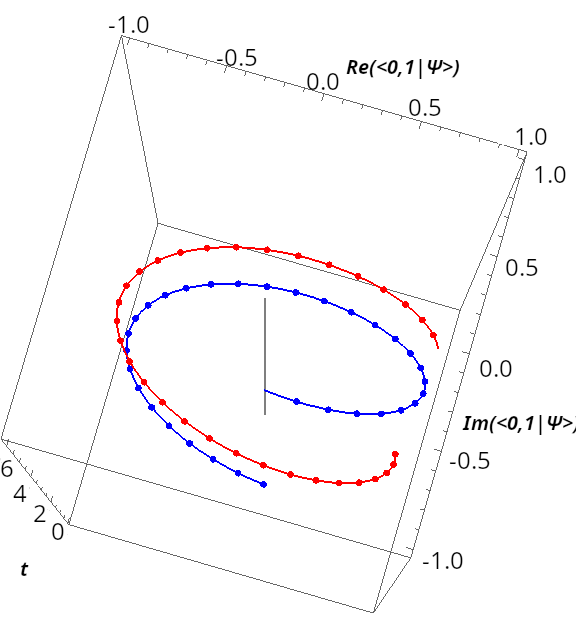
\includegraphics[width=0.22\textwidth]{PWfit32top-largelabels.png}
  \end{center}
  \caption{
    \color{Green}
    Comparison of discrete PaW model prediction (points) with the ordinary QM Schr\"odinger solution (continuous line).
    Complex values.
  }
\end{wrapfigure}

The frequency operator in $\hilb{H}_T$, as the canonically conjugate operator
of $\hat{T}$ in a finite-dimensional Hilbert space, is derived via
\emph{discrete Fourier transformation} \cite{FiniteHilb} (with $F_N$ unitary):
\begin{equation}
  \boxed{
    \hat{\Omega} = \frac{N}{2\pi} F^{}_{N} \hat{T} F^{\dagger}_{N}
  }
  \; \text{.}
\end{equation}
%
We therefore need to find the eigenvectors of $\hat{\mathbb{J}}$ as in \eqref{eq:pwHamiltonian}.
Such eigensolutions
will encode the whole (periodic) evolution of the qubit (in $\hilb{H}_S$), but do
not ``evolve'' themselves (as there's no external ``time'' outside $\hilb{H}_T \ox \hilb{H}_S$).

In our example, we take $N = 32$ and resolve numerically.
With the chosen $\hat{H}_S$,
of some interest are solutions that show
Rabi oscillation / Larmor precession,
i.e. solutions that do not correspond to eigenstates of
the ``ordinary'' Hamiltonian $\hat{H}_S$ of the qubit.
%
We pick $\dket{\Phi_{41}}$ corresponding to eigenvalue
$\epsilon_{41} = 11$.

The first two components
are interpreted as the components of the qubit in $\hilb{H}_S$ at $t=0$.
In general, the components
$2k$\nobreakdash-th and $2k+1$\nobreakdash-th
are compared to the components of the qubit at $k$-th discrete temporal step ($t = k \frac{2\pi}{N}$).

% \begin{center}\vspace{0.5cm}
%   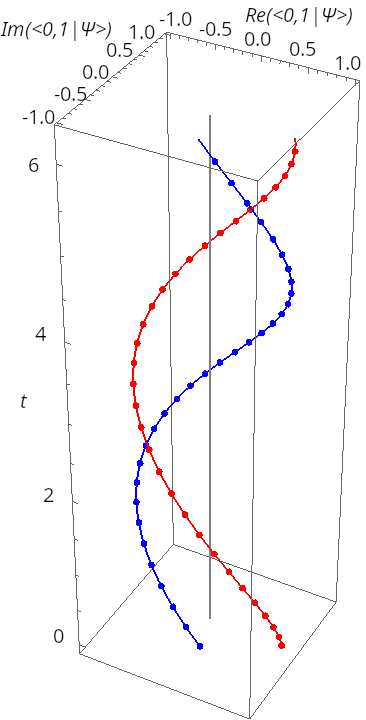
\includegraphics[width=0.15\linewidth]{PWfit32-largelabels.png}
%   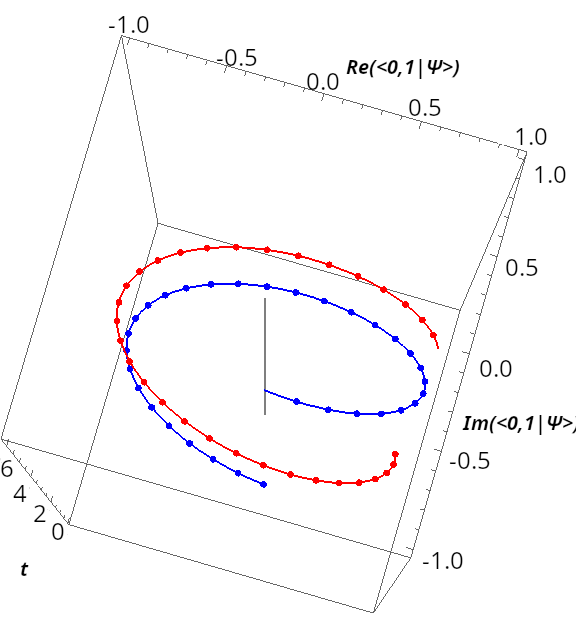
\includegraphics[width=0.25\linewidth]{PWfit32top-largelabels.png}
%   \captionof{figure}{
%     \color{Green}
%     Comparison of discrete PaW model prediction (points) with the ordinary QM Schr\"odinger solution (continuous line).
%     Complex values. 3-D plot shown on two angles.
%   }
% \end{center}

\section*{Application: Qutrit, absorptive detector, $N=60$-level clock}

\begin{wrapfigure}[13]{r}{0.25\textwidth}
  \begin{center}
    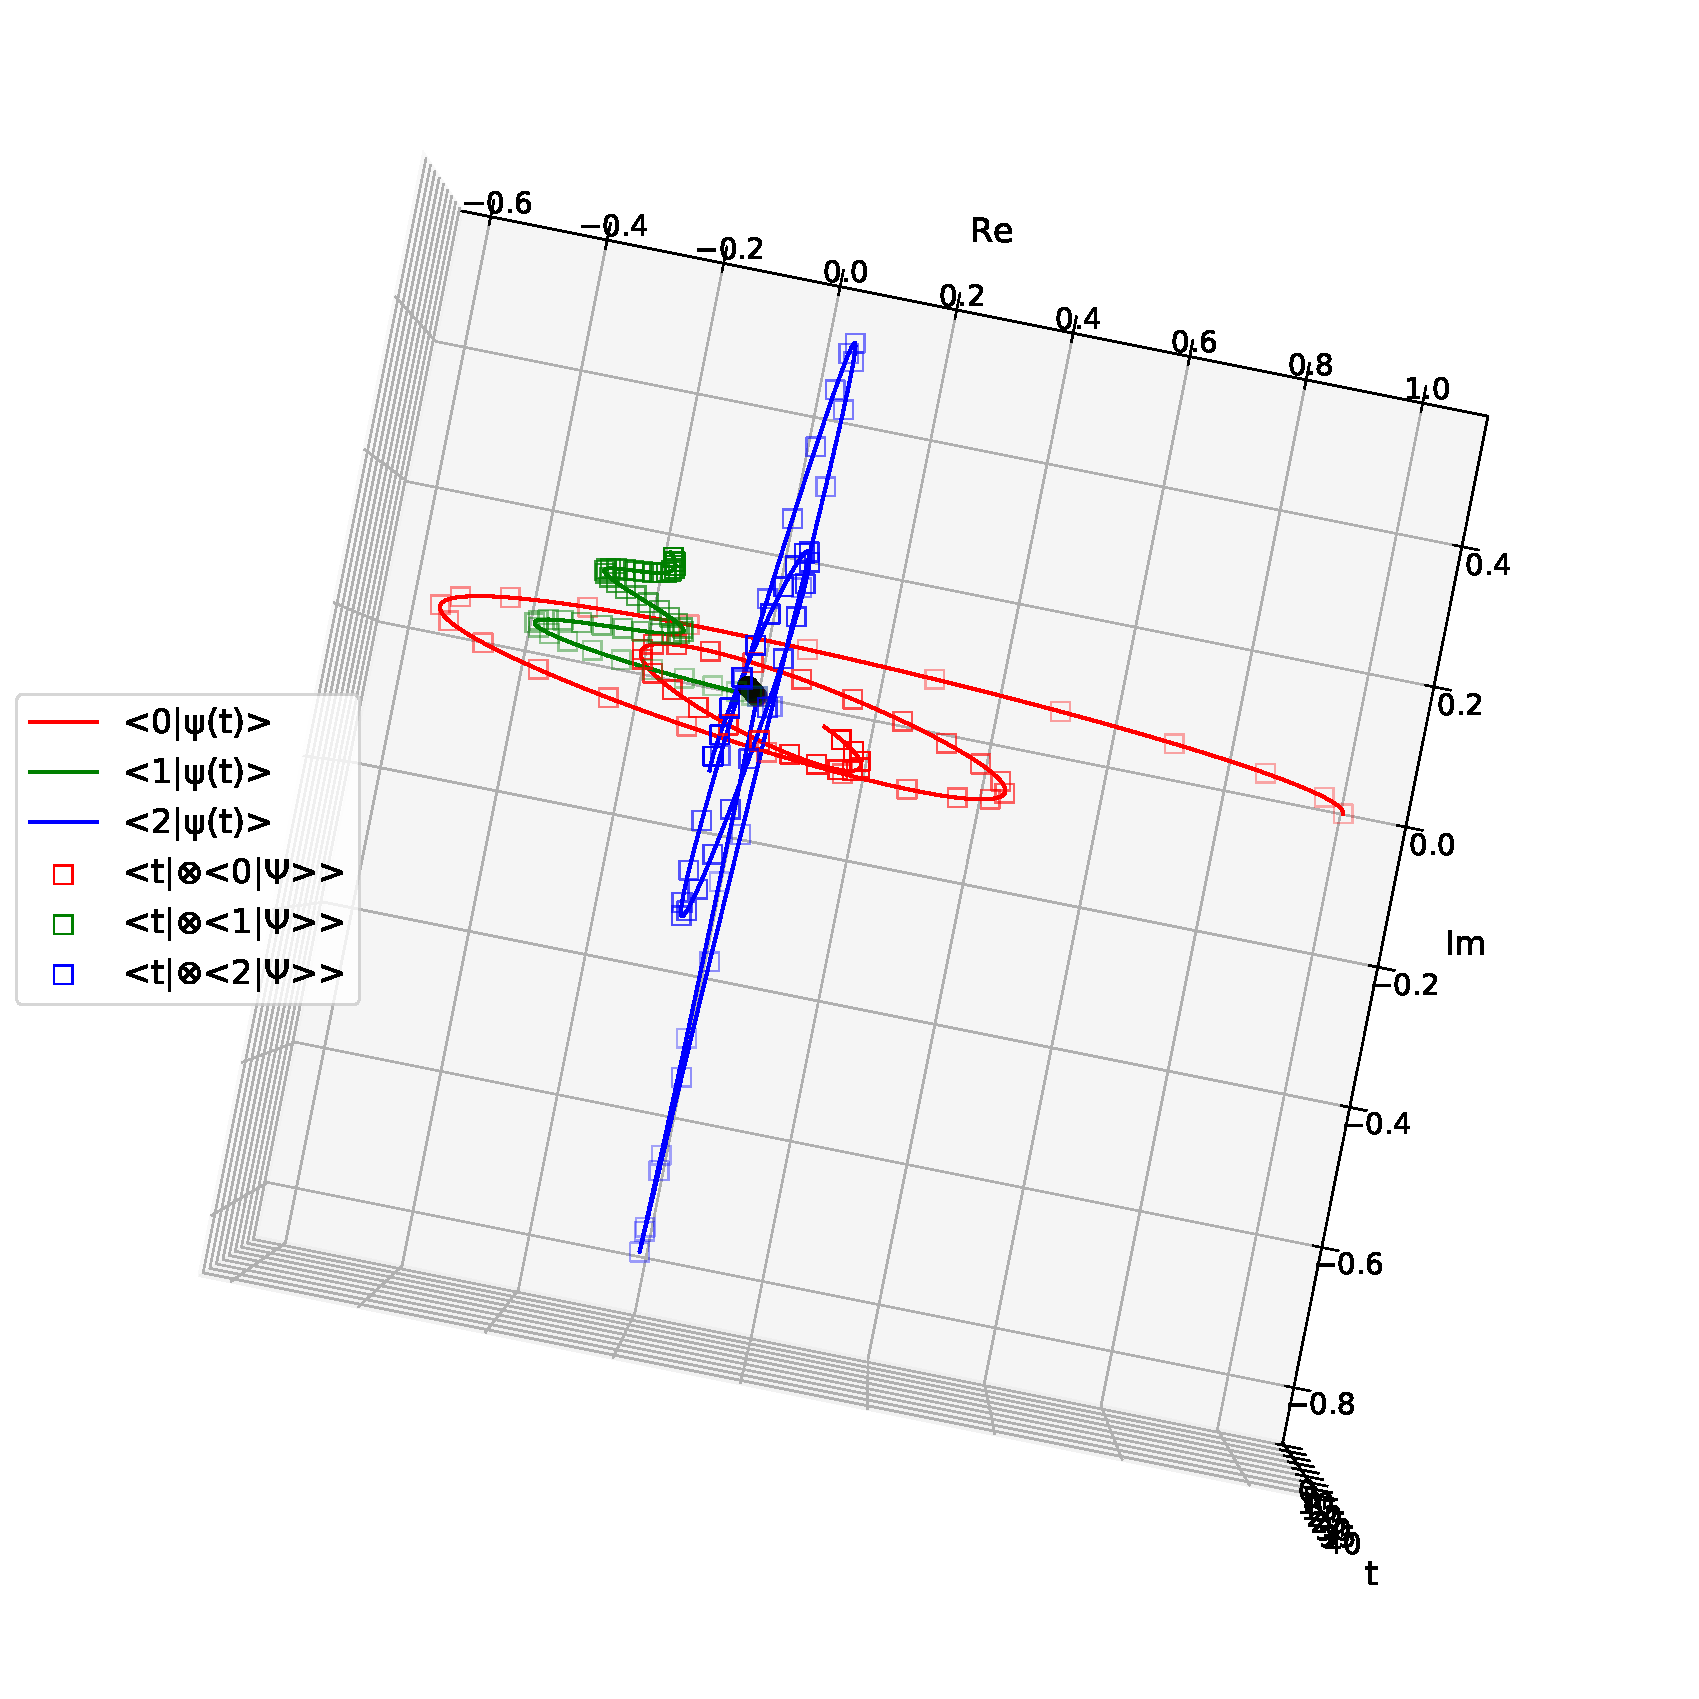
\includegraphics[width=0.25\textwidth]{3ldetect/PWSpaceTimeFit_top.pdf}
  \end{center}
  \caption{
    \color{Green}
    Non-unitary (absorptive) evolution of a 3-level system.
    Comparison of discrete PaW prediction (points) with the detector-model, ``Schr\"odinger'' solution (continuous line).
    Complex values.
  }
\end{wrapfigure}


Plugging the absoption term \cite{RuschhauptAbsorption}, $-i \op{D}_S$, hence non-unitary evolution, in the Page--Wootters Hamiltonian:
\begin{equation*}\label{eq:pwHamiltonian:nonUnitary}
  \op{\mathbb{J}} = \hbar\op{\Omega}\ox\idop_S + \idop_T\ox\qty(\op{H}_S -i \op{D}_S) \,\text{.}
\end{equation*}
Detection probability according to detector models, $-\dv{\norm{\psi}^2}{t}$, is compared with Page-Wootters
time of arrival probability distribution obtained in terms of (conditional) Bayesian theory:
\begin{multline*}\label{eq:3lev:bayesPW}
  P^{PW}(t_n|2) := P^{PW}\Big( t_n \Big| 2, \left[0,\Delta{T}\right]\Big) \\
  = \frac{
    \abs{\bra{t_n} \ox \bra{2} \cdot \dket{\Psi}}^2
  }{
    \sum_{n'=0}^{N_{T} - 1} \abs{\bra{t_{n'}} \ox \bra{2} \cdot \dket{\Psi}}^2
  }
  \,\text{,}
  \\
  \text{ where } t_{n'} = n'\delta{T} = \frac{n'\Delta{T}}{N_{T}}
  \text{.}
\end{multline*}

\vspace{10cm}

\begin{center}
  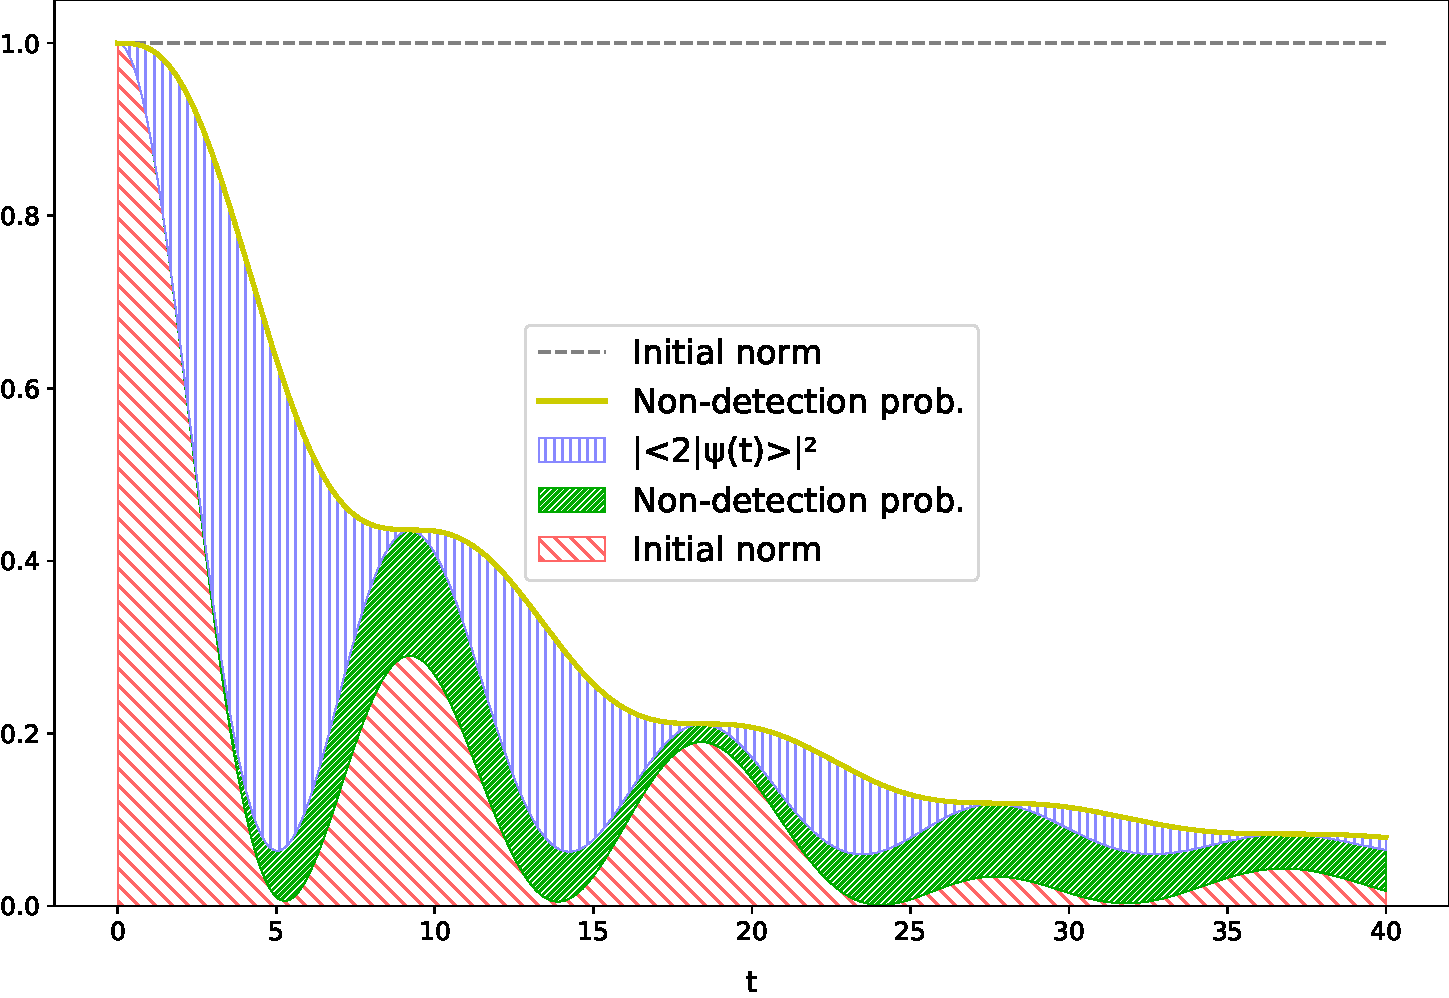
\includegraphics[width=.23\textwidth]{3ldetect/loss3color.pdf}
  \hspace{0.4cm}
  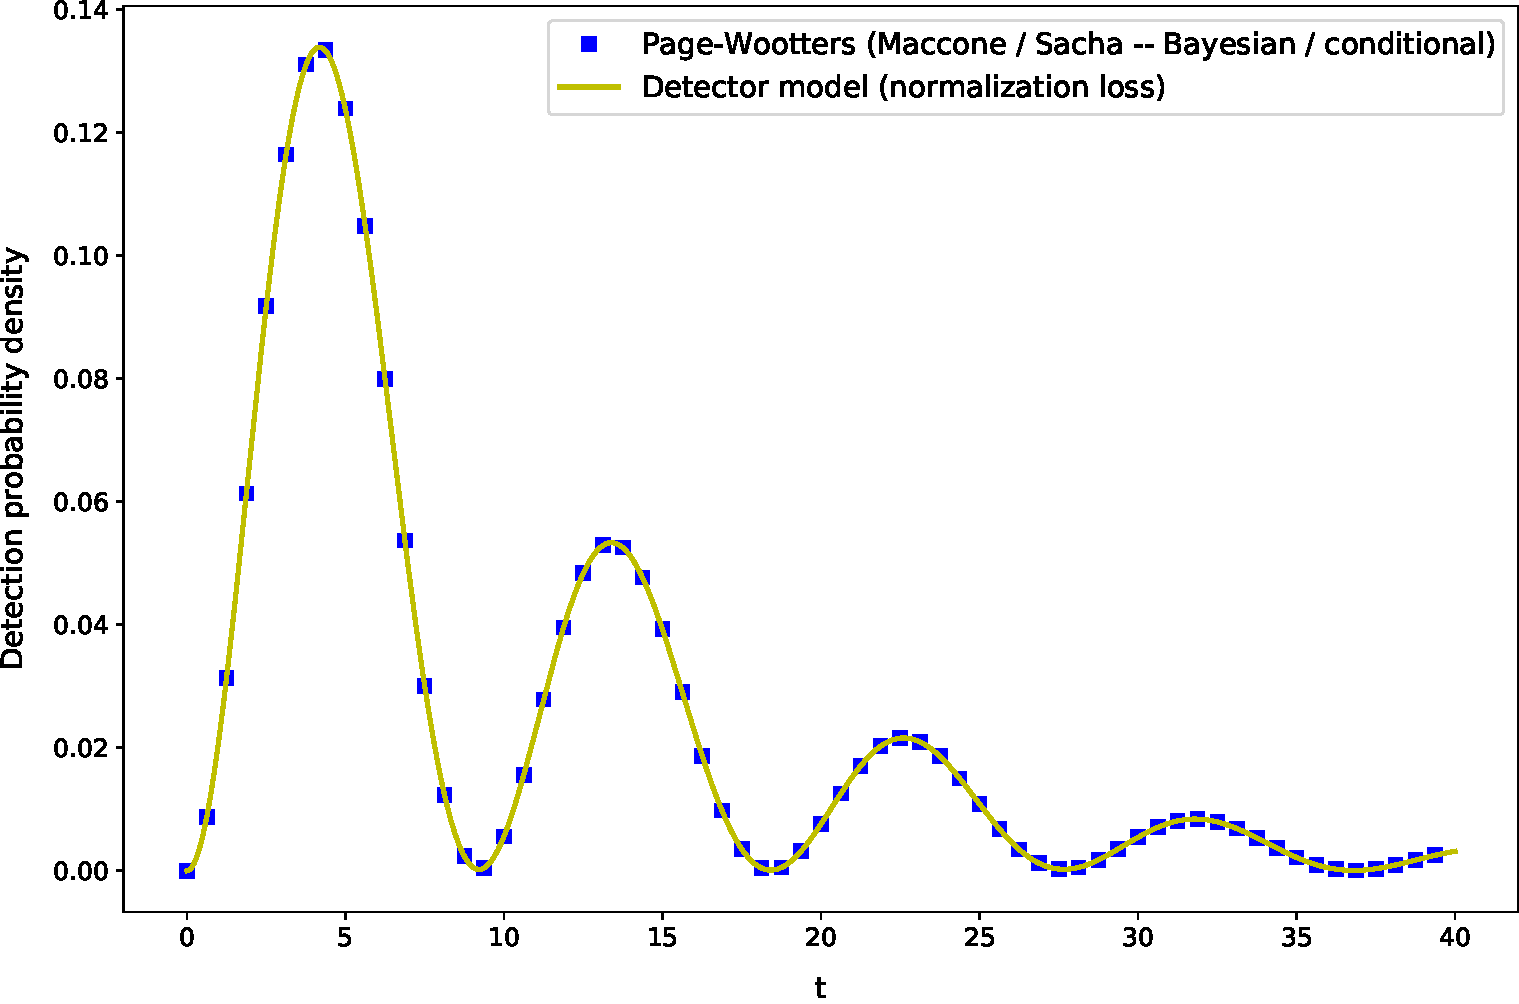
\includegraphics[width=.23\textwidth]{3ldetect/conditionalProbFit.pdf}
  \captionof{figure}{
    \color{Green}
    Normalization losss and detection probability.
  }
\end{center}
% \begin{center}\vspace{1cm}
%   %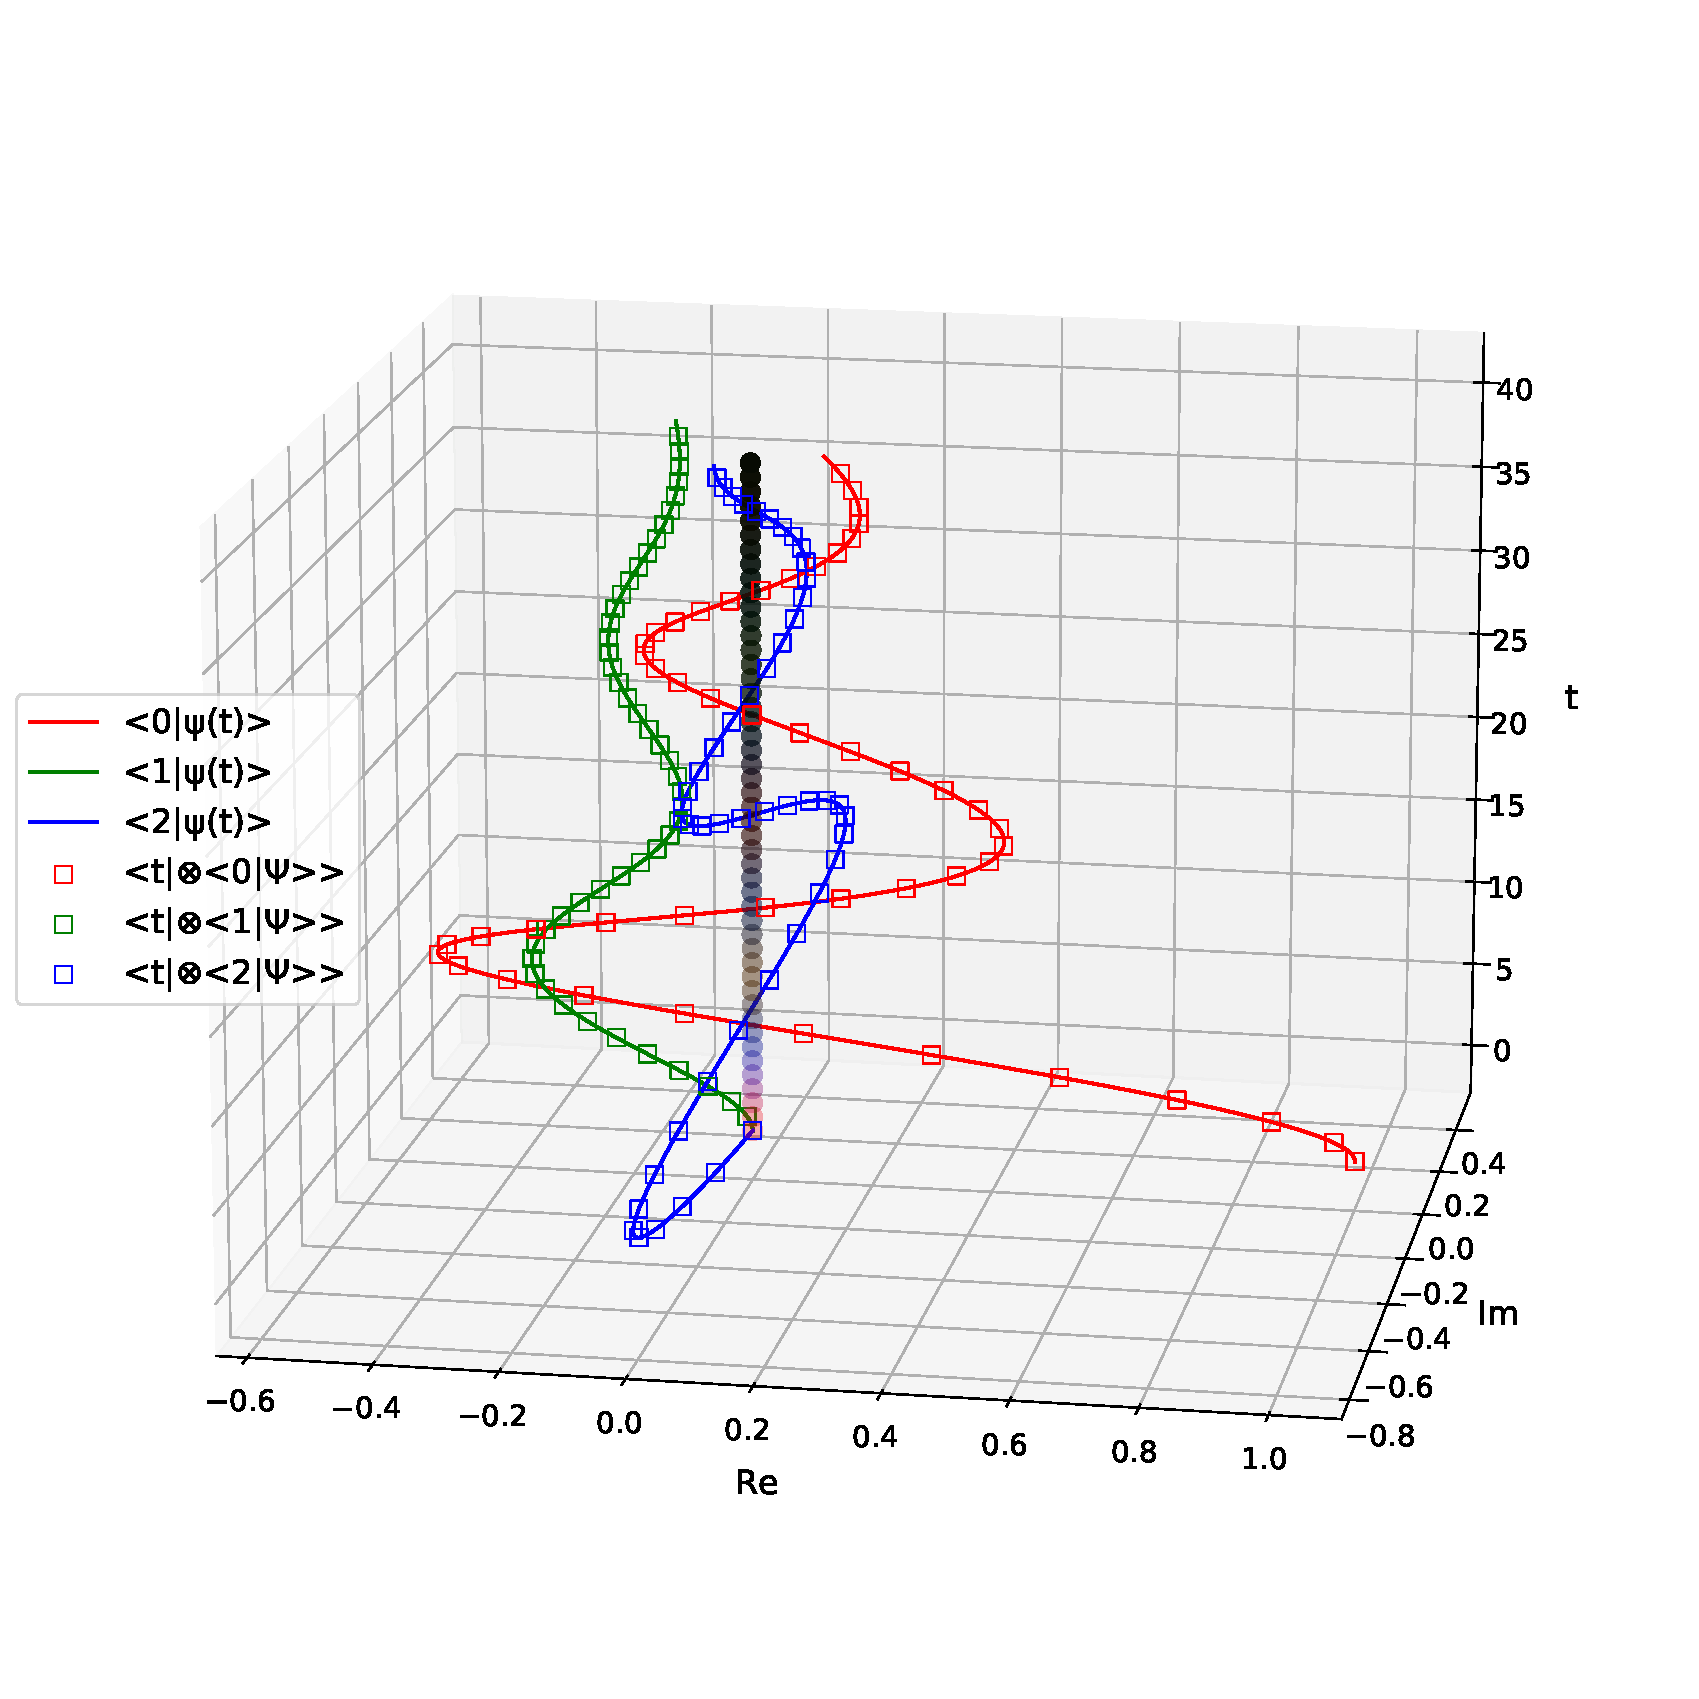
\includegraphics[width=.25\textwidth]{3ldetect/PWSpaceTimeFit_side.pdf}
%   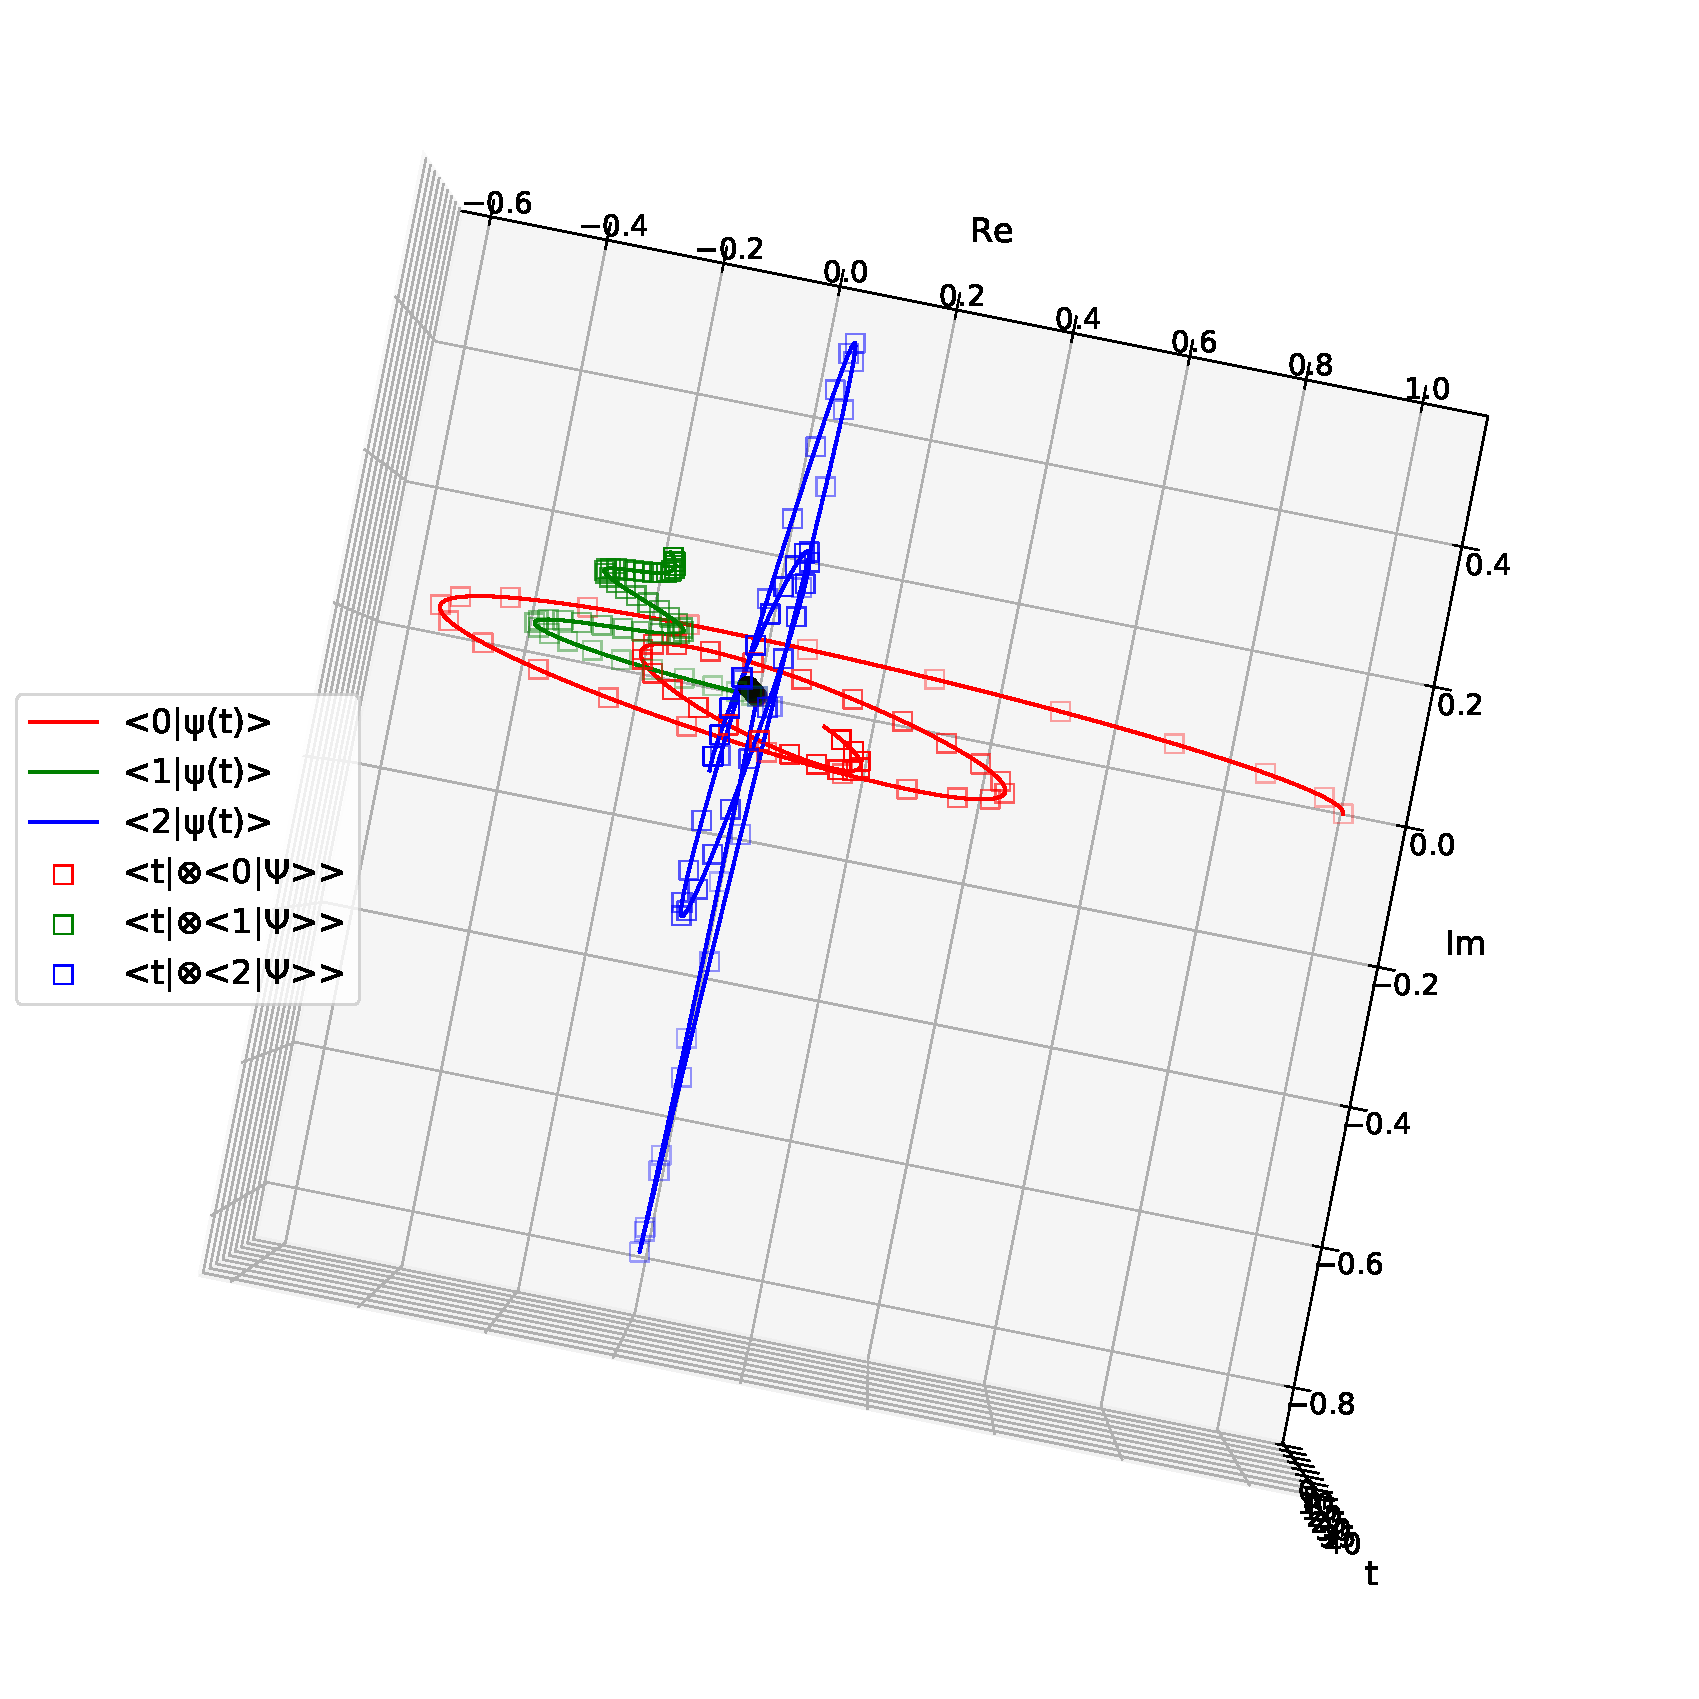
\includegraphics[width=.3\textwidth]{3ldetect/PWSpaceTimeFit_top.pdf}
%   \captionof{figure}{
%     \color{Green}
%     Discrete Page--Wootters results (points)
%     compared to continuous
%     Schr\"{o}dinger
%     evolution (continuous lines). Complex values.
%     %3-D plot shown on two angles.
%   }
% \end{center}

%----------------------------------------------------------------------------------------
%	CONCLUSIONS
%----------------------------------------------------------------------------------------

\color{SaddleBrown} % SaddleBrown color for the conclusions to make them stand out


% \section*{Conclusions and Outlook}

% \begin{itemize}
% \item Pellentesque eget orci eros. Fusce ultricies, tellus et pellentesque fringilla, ante massa luctus libero, quis tristique purus urna nec nibh. Phasellus fermentum rutrum elementum. Nam quis justo lectus.
% \item Vestibulum sem ante, hendrerit a gravida ac, blandit quis magna.
% \item Donec sem metus, facilisis at condimentum eget, vehicula ut massa. Morbi consequat, diam sed convallis tincidunt, arcu nunc.
% \item Nunc at convallis urna. isus ante. Pellentesque condimentum dui. Etiam sagittis purus non tellus tempor volutpat. Donec et dui non massa tristique adipiscing.
% \end{itemize}

\color{DarkSlateGray} % Set the color back to DarkSlateGray for the rest of the content

 %----------------------------------------------------------------------------------------
%	REFERENCES
%----------------------------------------------------------------------------------------

\printbibliography

%----------------------------------------------------------------------------------------
%	ACKNOWLEDGEMENTS
%----------------------------------------------------------------------------------------

% \section*{Acknowledgements}

% Etiam fermentum, arcu ut gravida fringilla, dolor arcu laoreet justo, ut imperdiet urna arcu a arcu. Donec nec ante a dui tempus consectetur. Cras nisi turpis, dapibus sit amet mattis sed, laoreet.

%----------------------------------------------------------------------------------------

\end{multicols}
\end{document}
